\section{Auswertung}
\label{sec:Auswertung}

\subsection{Zeitabhängigkeit der Amplitude}
\label{sec:Zeitabhängigkeit der Amplitude}
Aus dem Ozilloskopbild (\autoref{fig:aufgabe a}) wird die Höhe der einzelnen Peaks abgelesen und in \autoref{tab:Aufgabe a} festgehalten. Der 
zeitliche Abstand zwischen den Peaks wird zu $\qty{27,27}{\micro\second}$ bestimmt.

\begin{figure} [H]
  \centering
  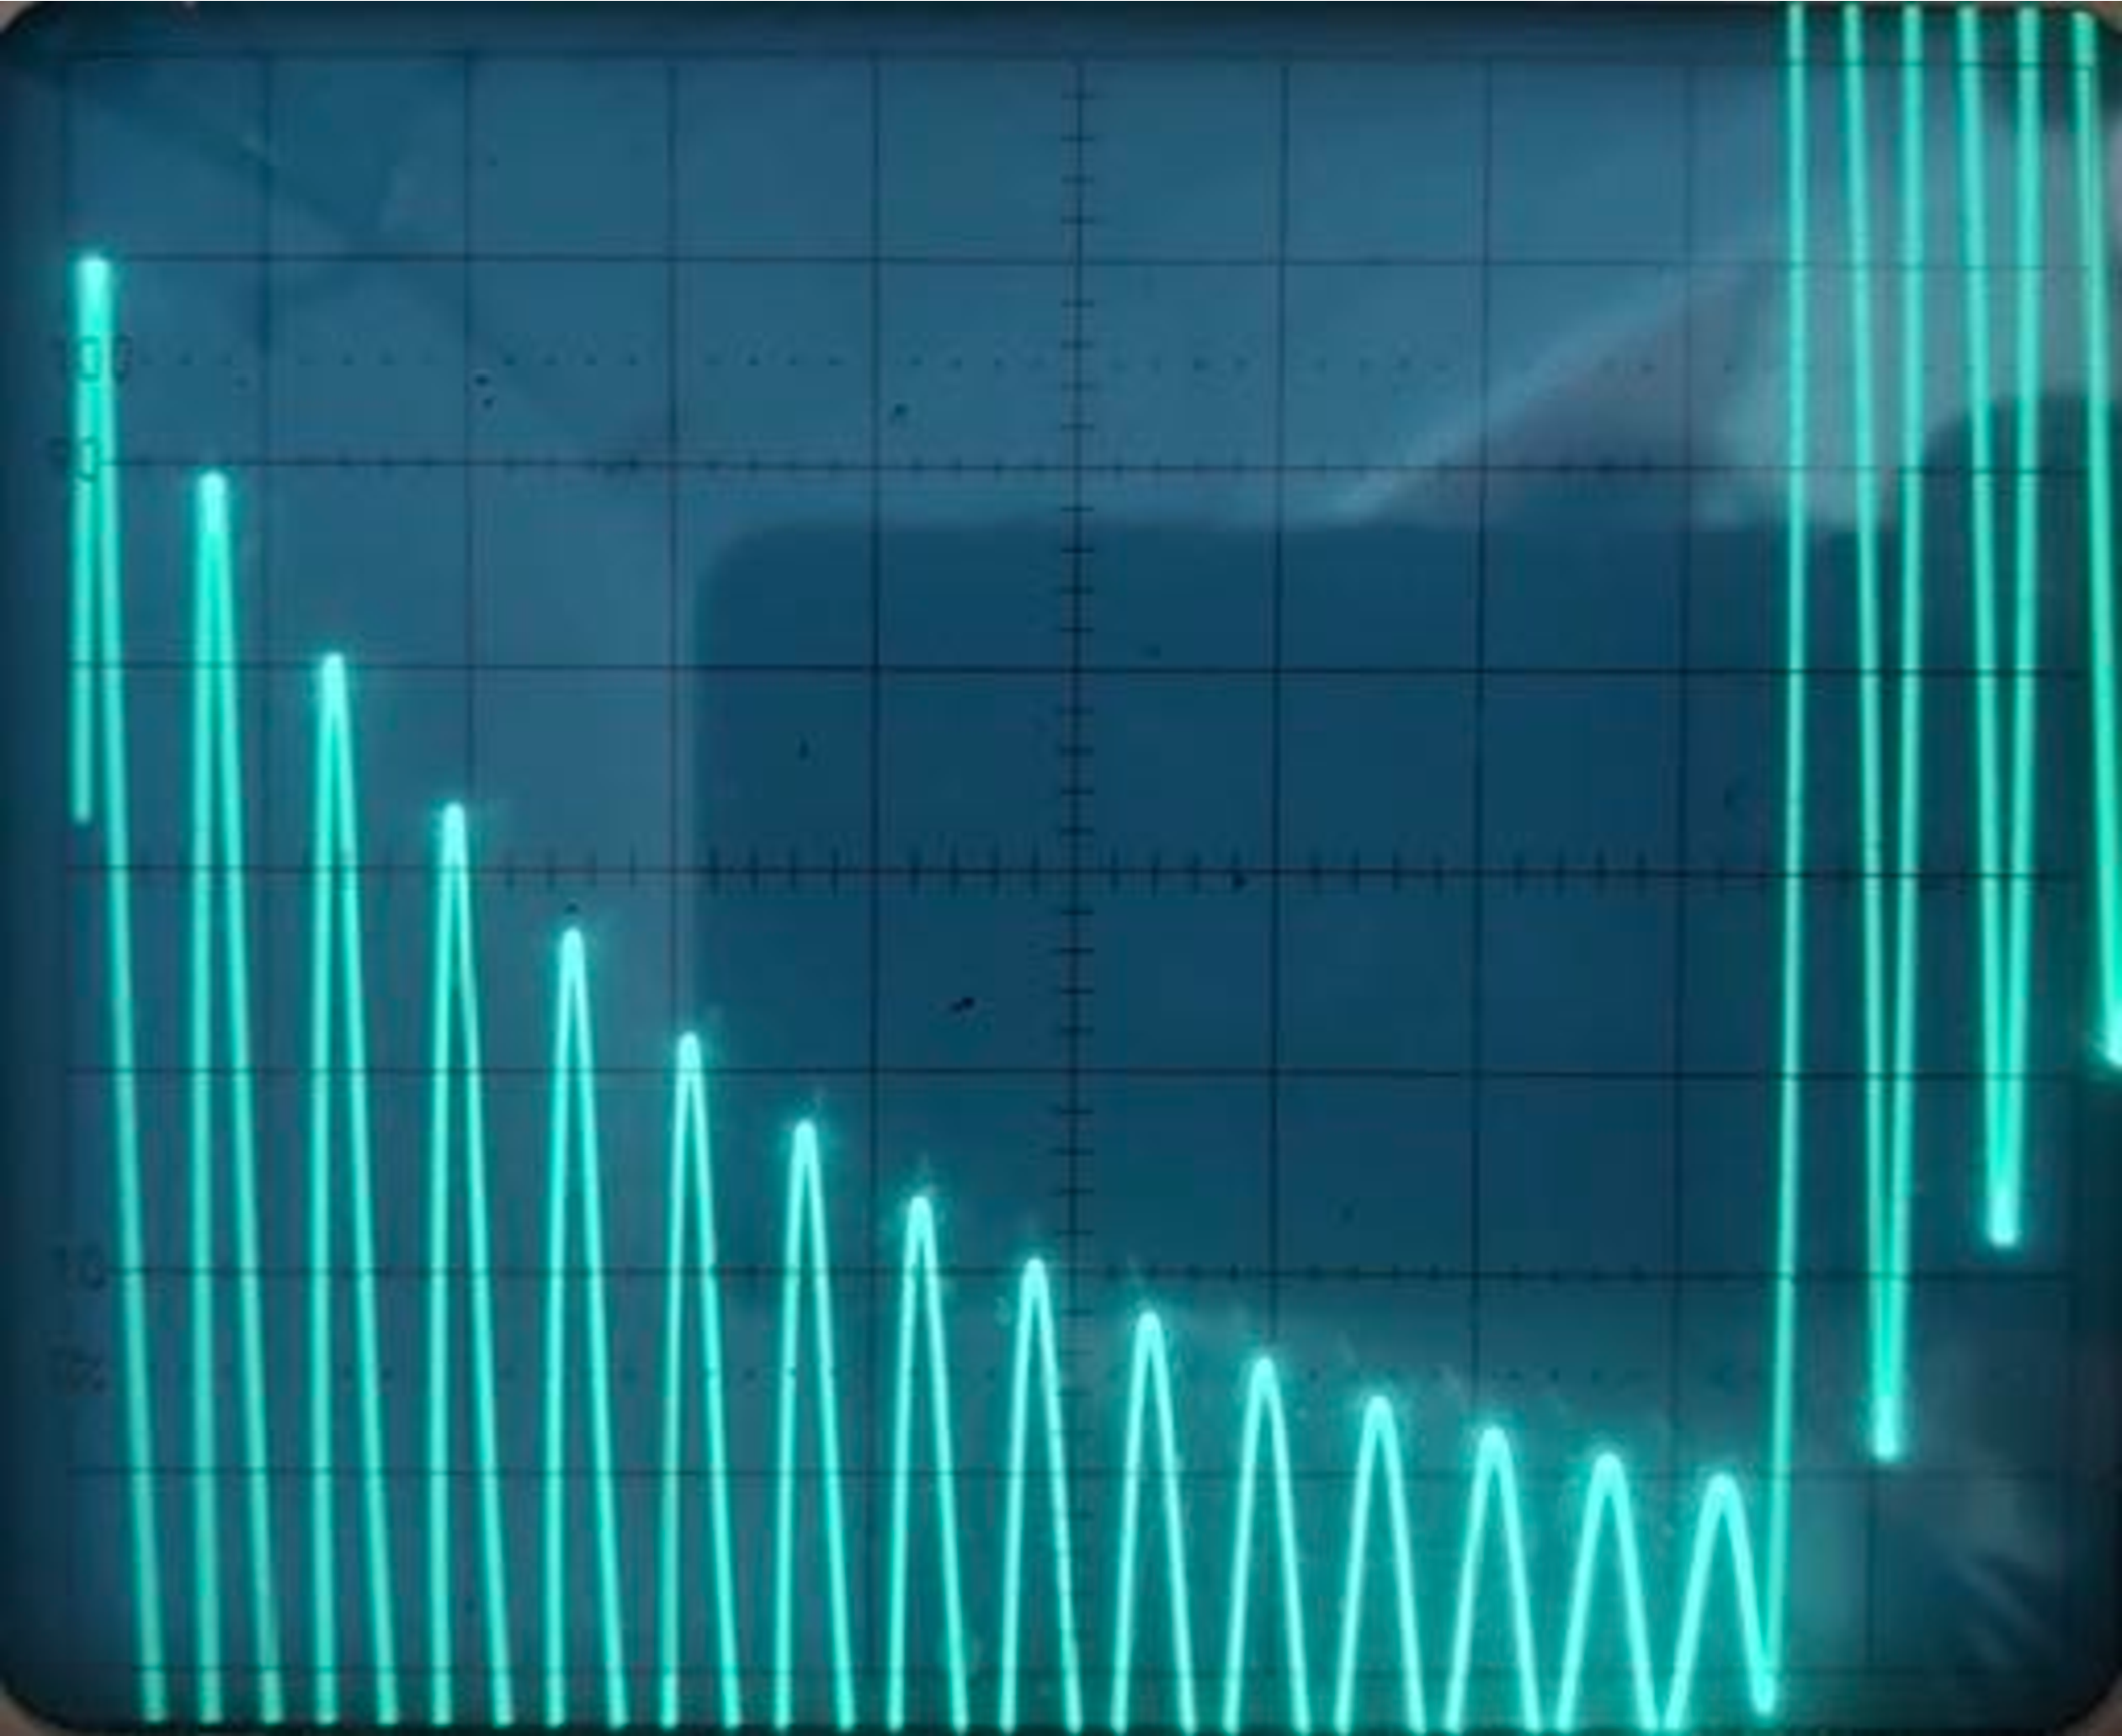
\includegraphics[height=10cm]{content/Bilder/Aufgabe_a.pdf}
  \caption{Bild des Oszilloskopbildschirms aus dem die Höhe der Amplituden der einzelnen Peaks abgelesen wird.}
  \label{fig:aufgabe a}
\end{figure}

\begin{table}
  \centering
  \caption{Amplitude der einzelnen Peaks aus \autoref{fig:aufgabe a} mit einem zeitlichen Abstand von $\qty{27,27}{\micro\second}$.}
  \label{tab:Aufgabe a}
  \begin{tabular}{S[table-format=1.1]}
    \toprule
    {$U\,/\,\unit{\volt}$} \\
    \midrule
    6.0 \\
    5.0 \\
    4.1 \\
    3.3 \\
    2.7 \\
    2.2 \\
    1.8 \\
    1.4 \\
    1.1 \\
    0.8 \\
    0.5 \\
    0.4 \\
    0.2 \\
    0.1 \\
    \bottomrule
  \end{tabular}
\end{table}

Die Messwerte werden graphisch dargestellt. Für die logarithmische Darstellung der Messwerte $\frac{U}{U_0}$ mit dem Wert $U_0=\qty{6}{\volt}$
wird mit der Python-Erweiterung \textit{scipy} \cite{scipy} eine lineare Ausgleichsrechnung durchgeführt und es ergibt sich die Ausgleichsgerade
\begin{equation}
  \ln(\frac{U}{U_0})=\qty{-0,0106+-0,0007}{\per\micro\second} \cdot t + (0,3013\pm0,0007).
  \label{eq:Ausgleichsgerade}
\end{equation}

\begin{figure} [H]
  \centering
  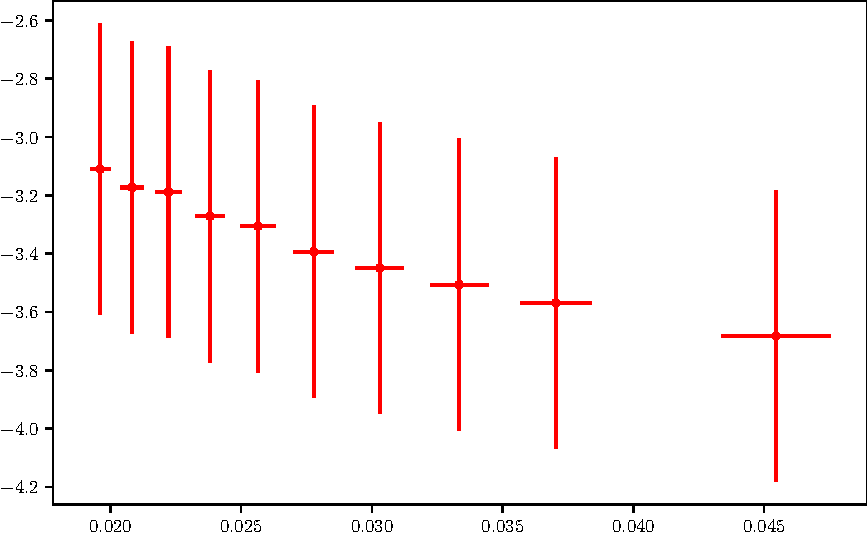
\includegraphics{build/plot_a.pdf}
  \caption{Zeitabhängigkeit der Spannung}
  \label{fig:plot_a}
\end{figure}

% Effektiver Widerstand %
\subsubsection{Effektiver Widerstand $R_{\symup{eff}}$}
Um den effektiven Widerstand des Schwingkreises herauszufinden, wird \eqref{eq:effektiver Widerstand} verwendet. Der Faktor $2\symup{\pi}\mu$ ergibt
sich als Steigung der Ausgleichsgeraden \eqref{eq:Ausgleichsgerade}:
\begin{equation*}
  R_{\symup{eff, experiment}}=\qty{214+-14}{\ohm}.
\end{equation*}
Der theoretisch zu bestimmende Effektivwiderstand $R_{\symup{eff, theorie}}$ setzt sich aus dem verwendeten Widerstand $R_1$ und dem
Innenwiderstand des Frequenzgenerators von etwa $\qty{50}{\ohm}$ zusammen zu
\begin{equation*}
  R_{\symup{eff, theorie}} = \qty{98.10+-0.10}{\ohm}.
\end{equation*}

% Abklingzeit %
\subsubsection{Abklingzeit $T_{\symup{ex}}$}
Nach \ref{eq:Abklingzeit} ergibt sich die experimentell ermittelte Abklingzeit zu
\begin{equation*}
  T_{\symup{ex, experimentell}} = \qty{95+-6}{\micro\second}.
\end{equation*}
Ebenfalls mithilfe von \ref{eq:Abklingzeit} wird der theoretische Wert der Abklingzeit bestimmt zu
\begin{equation*}
  T'_{\symup{ex, theoretisch}} = \qty{206.12}{\micro\second}.
\end{equation*}
Die Messunsicherheit von $T_{\symup{ex, theoretisch}}$ wird mithilfe der gaußschen Fehlerfortpflanzung bestimmt
\begin{align*}
  \symup{\Delta}T_{\symup{ex, theoretisch}} &= \sqrt{\Bigl(\frac{\symup{d}T_{\text{ex}}}{\symup{d}L}\symup{\Delta} L \Bigr)^2+
  \Bigl(\frac{\symup{d}T_{\text{ex}}}{\symup{d}R}\symup{\Delta} R\Bigr)^2} \\
  &=\sqrt{\Bigl(\frac{2}{R}\symup{\Delta} L\Bigr)^2+\Bigl(\frac{-2L}{R^2}\symup{\Delta}R\Bigr)^2} \\
  &\approx \qty{0.21}{\micro\second}
\end{align*}
Für die theoretische Abklingzeit $T_{\symup{ex, theoretisch}}$ ergibt sich folglich der Wert
\begin{equation*}
  T_{\symup{ex, theoretisch}} = \qty{206.12+-0.21}{\micro\second}.
\end{equation*}

%%%%% Aperiodischer Grenzfall %%%%%
\subsection{Aperiodischer Grenzfall}
\label{sec:Aperiodischer Grenzfall}

Nach der Vorgehensweise aus \ref{sec:Aperiodischer Grenzfall Durchführung} ergibt sich für den gesuchten Widerstand \\
\begin{gather*}
  R_{\symup{ap}} = \qty{3,40+-0.01}{\kilo\ohm}. \\ \notag
\end{gather*}

Als Referenz wird außerdem der theoretische Wert berechnet, der sich aus \eqref{eq:Widerstand aperiodischer Grenzfall} ergibt.
Dessen Fehler bestimmt sich mit der gaußschen Fehlerfortpflanzung zu:

\begin{align*}
  \label{eqn:Fehler Rap}
  \symup{\Delta} R_{\text{ap}} &= \sqrt{\Bigl(\frac{\symup{d}R_{\text{ap}}}{\symup{d}L}\symup{\Delta} L \Bigr)^2+\Bigl(\frac{\symup{d}R_{\text{ap}}}{\symup{d}C}\symup{\Delta} C\Bigr)^2} \\
  &= \sqrt{\Bigl(\frac{1}{\sqrt{LC}}\symup{\Delta} L\Bigr)^2+\Bigl(\frac{\sqrt{LC}}{C^2}\symup{\Delta} C\Bigr)^2} \\
  &\approx 7\,\unit{\ohm}
\end{align*}

Insgesamt erhält man also aus der Theorie:
\begin{gather*}
  R_{\symup{ap, theoretisch}} = \qty{4,396+-0.007}{\kilo\ohm}. \\ \notag
\end{gather*}

\subsection{Frequenzabhängigkeit der Spannung}
\label{sec:Frequenzabhängigkeit der Spannung}

In \autoref{tab:Aufgabe c} ist die frequenzabhängige Spannungsamplitude des Frequenzgenerators $U_0$ und des Ausgangssignals $U$
aufgeführt. Es wird im weiteren Verlauf mit dem Verhältnis $\frac{U}{U_{0}}$ gearbeitet, damit sich eine mögliche
Frequenzabhängigkeit von $U_0$ relativiert und das Ergebnis nicht verfälscht. 

Zuerst wird $\frac{U}{U_{0}}$ in \autoref{fig:plot_c} halblogarithmisch gegen die Frequenz geplottet.
Zusätlich wurde hier noch zur Übersichtlichkeit der theoretische Verlauf, der durch \eqref{eq:Spannung} beschrieben wird, eingefügt.

Es lässt sich aus \autoref{fig:plot_c} nun die Resonanzüberhöhung $q_{\symup{exp}}$ entnehmen, diese entspricht dem größten Messwert bzw.
dem experiementellen Maximum:
\begin{gather*}
  q_{\symup{exp}} = 3,9\,\unit{\volt}. \notag
\end{gather*}

Anschließend soll die Breite der Resonanzkurve bestimmt werden.
Dafür wird der Spannungsverlauf im Resonanzbereich in \autoref{fig:plot_c_2} linear geplottet.
Damit werden entsprechend \eqref{eq:Breite Resonanzkurve} $f_+$ und $f_-$ als die Frequenzen bestimmt, bei denen
die Spannung auf das  $\frac{1}{\sqrt{2}}$-Fache des Maximums abgefallen ist.
Aus deren Differenz ergibt sich dann die Breite der Resonanzkurve experiementell zu
\begin{gather*}
  \symup{\Delta}f_{\symup{exp}} = 37,7\,\unit{\kilo\hertz} - 28,9\,\unit{\kilo\hertz} = 8,8\,\unit{\kilo\hertz}. \notag
\end{gather*}

Als nächstes werden die ermittelten Werte mit den theoretischen Werten verglichen.
Die Breite der Resonanzkurve kann nach \eqref{eq:Breite Resonanzkurve} abgeschätzt werden zu
\begin{gather*}
  \symup{\Delta}f_{\symup{theorie}} = \qty{8.808+-0.008}{\kilo\hertz} \notag
\end{gather*}
und steht somit in guter Übereinstimmung mit dem experiementellen Ergebnis.

Die Resonanzüberhöhung lässt sich ebenfalls mit \eqref{eq:Güte} theoretisch berechnen und lautet
\begin{gather*}
  q_{\symup{theorie}} = \qty{3.928+-0.003}{\volt}. \notag
\end{gather*}
Also kann auch hier eine gute Übereinstimmung von Theorie und Experiement festgestellt werden.

\begin{table} [H]
  \centering
  \caption{Messwertpaare der zur Frequenz $f$ zugehörigen Amplituden $U_{0}$, $U$ sowie der Relativamplitude $\frac{U}{U_{0}}$.}
  \label{tab:Aufgabe c}
  \begin{tabular}{S[table-format=2.0] S[table-format=1.1] S[table-format=2.1] S[table-format=1.1]}
    \toprule
    {$f\,/\,\unit{\hertz}$} & {$U_{0}\,/\,\unit{\volt}$} & {$U\,/\,\unit{\volt}$} & {$\frac{U}{U_{0}}$} \\
    \midrule
    10 & 3.6 & 4.0  & 1.1 \\
    15 & 3.6 & 4.2  &	1.2 \\
    20 & 3.6 & 5.2  & 1.4 \\
    22 & 3.6 & 6.0  & 1.7 \\
    24 & 3.6 & 6.6  & 1.8 \\
    26 & 3.6 & 7.6  & 2.1 \\
    28 & 3.6 & 9.0  & 2.5 \\
    29 & 3.6 & 10.0 & 2.8 \\
    30 & 3.6 & 11.0 & 3.1 \\
    31 & 3.6 & 12.5 & 3.5 \\
    32 & 3.6 & 13.0 & 3.6 \\
    33 & 3.6 & 14.0 & 3.9 \\
    34 & 3.6 & 13.8 & 3.8 \\
    35 & 3.6 & 13.0 & 3.6 \\
    36 & 3.6 & 12.0 & 3.4 \\
    37 & 3.6 & 11.0 & 3.1 \\
    38 & 3.6 & 9.5  & 2.6 \\
    40 & 3.6 & 7.6  & 2.1 \\
    42 & 3.6 & 6.0  & 1.6 \\
    45 & 3.6 & 4.4  & 1.2 \\
    47 & 3.6 & 3.8  & 1.1 \\
    \bottomrule
  \end{tabular}
\end{table}

\begin{figure} [H]
  \centering
  \includegraphics{build/plot_c.pdf}
  \caption{Frequenzabhängigkeit der Spannung}
  \label{fig:plot_c}
\end{figure}

\begin{figure} [H]
  \centering
  \includegraphics{build/plot_c_2.pdf}
  \caption{Linearer Plot der Messwerte als Kurve im Resonanzbereich}
  \label{fig:plot_c_2}
\end{figure}

\subsection{Frequenzabhängigkeit der Phasenverschiebung}
\label{sec:Frequenzabhängigkeit der Phasenverschiebung}

Die Messwerte für $a$ und $b$ sind in \autoref{tab:aufgabe d} festgehalten.
Der Phasenversatz $\varphi$ wird daraus berechnet mit
\begin{equation}
  \varphi=\frac{2\pi a}{b}.
\end{equation}
In \autoref{fig:plot_d} sind diese Werte halblogarithmisch geplottet.
Es wurde zusätlich die Theoriekurve entsprechend \eqref{eq:Phasenverschiebung} eingefügt.

Anschließend wird der Bereich um $\varphi=\frac{\pi}{2}$ in \autoref{fig:plot_d_2} linear dargestellt.
Aus dieser Darstellung können nun die Werte für $f_{\symup{res}}$, $f_{1}$ und $f_{2}$ entnommen werden:
\begin{align*}
  f_{\symup{res, exp}} &= 34.3\,\unit{\kilo\hertz} \\
  f_{\symup{1,exp}} &= 30.4\,\unit{\kilo\hertz} \\
  f_{\symup{2,exp}} &= 39.4\,\unit{\kilo\hertz}.
\end{align*}

Mithilfe von \eqref{eq:Resonanzfrequenz}, \eqref{eq:omega 1} und \eqref{eq:omega 2} können diese Werte auch theoretisch bestimmt werden zu
\begin{align*}
  f_{\symup{res, theorie}} &= \qty{34.033+-0.001}{\kilo\hertz} \\
  f_{\symup{1,theorie}} &= \qty{30.473+-0.003}{\kilo\hertz} \\
  f_{\symup{2,theorie}} &= \qty{39.282+-0.004}{\kilo\hertz}.
\end{align*}
Hier zeigt sich ebenfalls eine gute Übereistimmung zwischen den theoretischen und experiementellen Werten.

\begin{table} [H]
  \centering
  \caption{Messwertepaare der von der Frequenz $f$ abhängigen
  Phasenverschiebung $\varphi$, die aus dem Phasenversatz $a$ und der Periodenlänge $b$ berechnet wird.}
  \label{tab:aufgabe d}
  \begin{tabular}{S[table-format=2.0] S[table-format=1.1] S[table-format=2.0] S[table-format=1.3]}
    \toprule
    {$f\,/\,\unit{\hertz}$} & {$a\,/\,\unit{\micro\metre}$} & {$b\,/\,\unit{\micro\metre}$} & {$\varphi$} \\
    \midrule
    10 & 1.0 & 98 & 0.064 \\ 
    15 & 1.0 & 75 & 0.083 \\
    20 & 1.2 & 49 & 0.153 \\
    22 & 1.6 & 44 & 0.228 \\
    24 & 1.8 & 41 & 0.275 \\
    26 & 2.2 & 38 & 0.363 \\
    28 & 2.8 & 35 & 0.502 \\
    29 & 3.4 & 34 & 0.628 \\
    30 & 3.8 & 33 & 0.723 \\
    31 & 4.4 & 32 & 0.863 \\
    32 & 5.0 & 31 & 1.013 \\
    33 & 6.0 & 30 & 1.256 \\
    34 & 7.0 & 29 & 1.516 \\
    35 & 7.8 & 29 & 1.689 \\
    36 & 8.4 & 28 & 1.884 \\
    37 & 9.0 & 27 & 2.094 \\
    38 & 9.2 & 26 & 2.223 \\ 
    40 & 9.6 & 25 & 2.412 \\
    42 & 9.7 & 24 & 2.539 \\ 
    45 & 9.6 & 22 & 2.741 \\
    47 & 9.6 & 21 & 2.872 \\
    \bottomrule
  \end{tabular}
\end{table}

\begin{figure} [H]
  \centering
  \includegraphics{build/plot_d.pdf}
  \caption{Frequenzabhängigkeit der Phasenverschiebung.}
  \label{fig:plot_d}
\end{figure}

\begin{figure} [H]
  \centering
  \includegraphics{build/plot_d_2.pdf}
  \caption{Linearer Plot der Messwerte als Kurve im Bereich um $\frac{\pi}{2}$.}
  \label{fig:plot_d_2}
\end{figure}